\Act*{4}
\Scene{1}[Before \textsc{Prospero's} cell.]


\begin{figure}[t!]
	\centering
	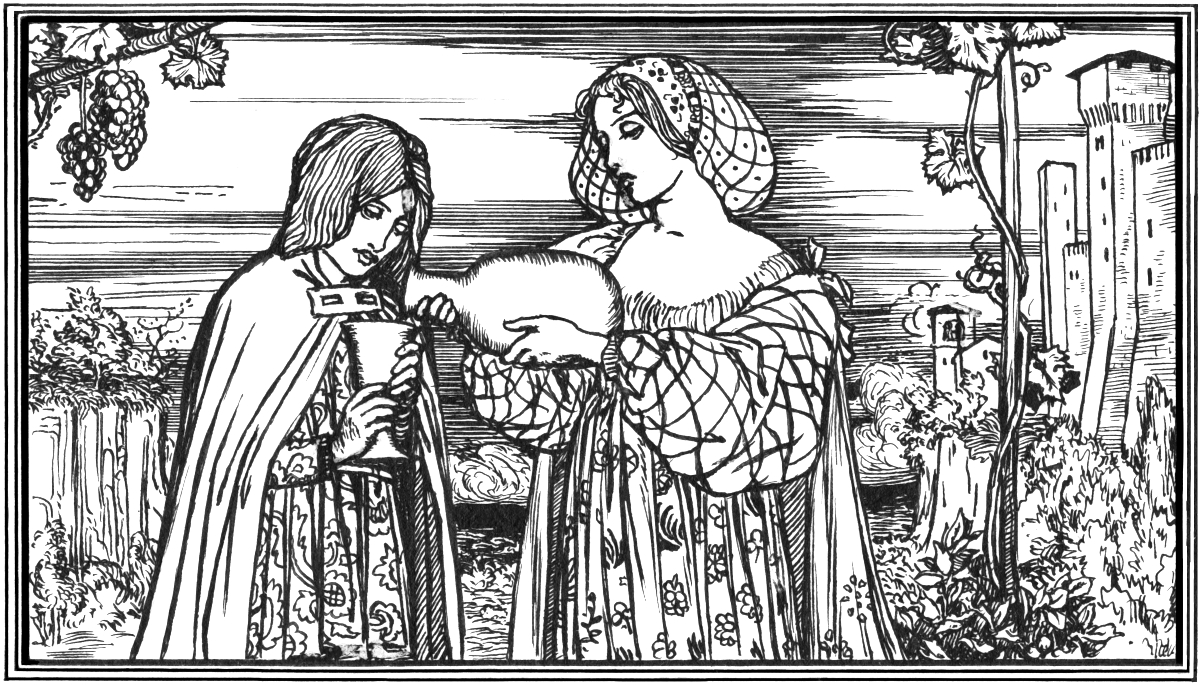
\includegraphics[width=\headerwidth]{4iheadpiece}
\end{figure}

\enter{\textsc{Prospero}, \textsc{Ferdinand}, and \textsc{Miranda}}

\begin{letter} %dropcap
	\begin{tikzpicture}[remember picture, overlay]
		\node (dropcap) at ($(current page.west)+(3cm,-3cm)$) {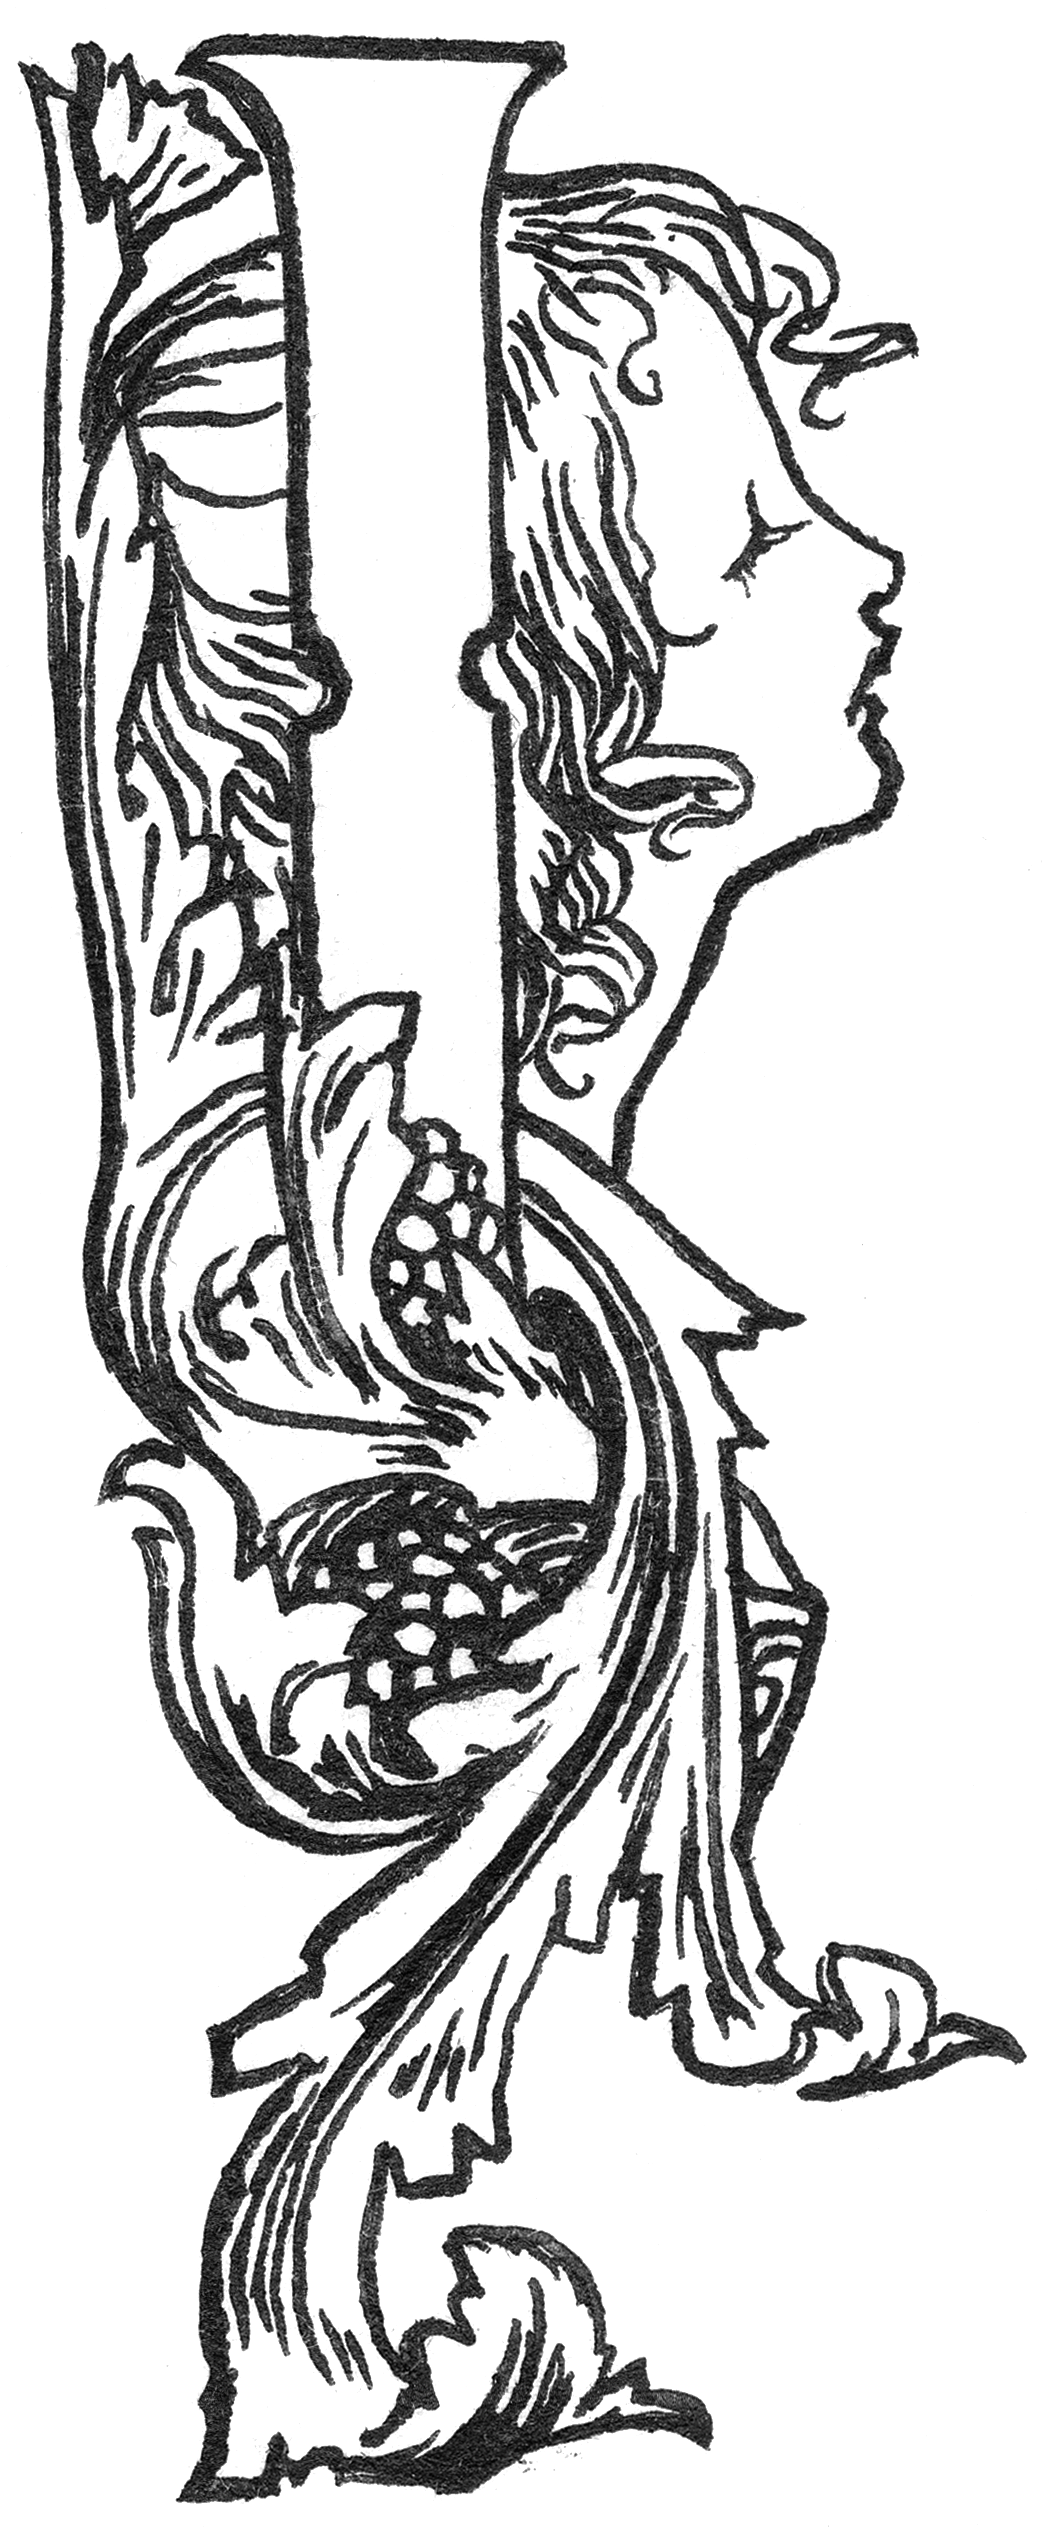
\includegraphics[width=0.125\linewidth]{4idropcapI}};
	\end{tikzpicture}
\end{letter}

\begin{a4} %dropcap
	\begin{tikzpicture}[remember picture, overlay]
		\node (dropcap) at ($(current page.west)+(3cm,-2.75cm)$) {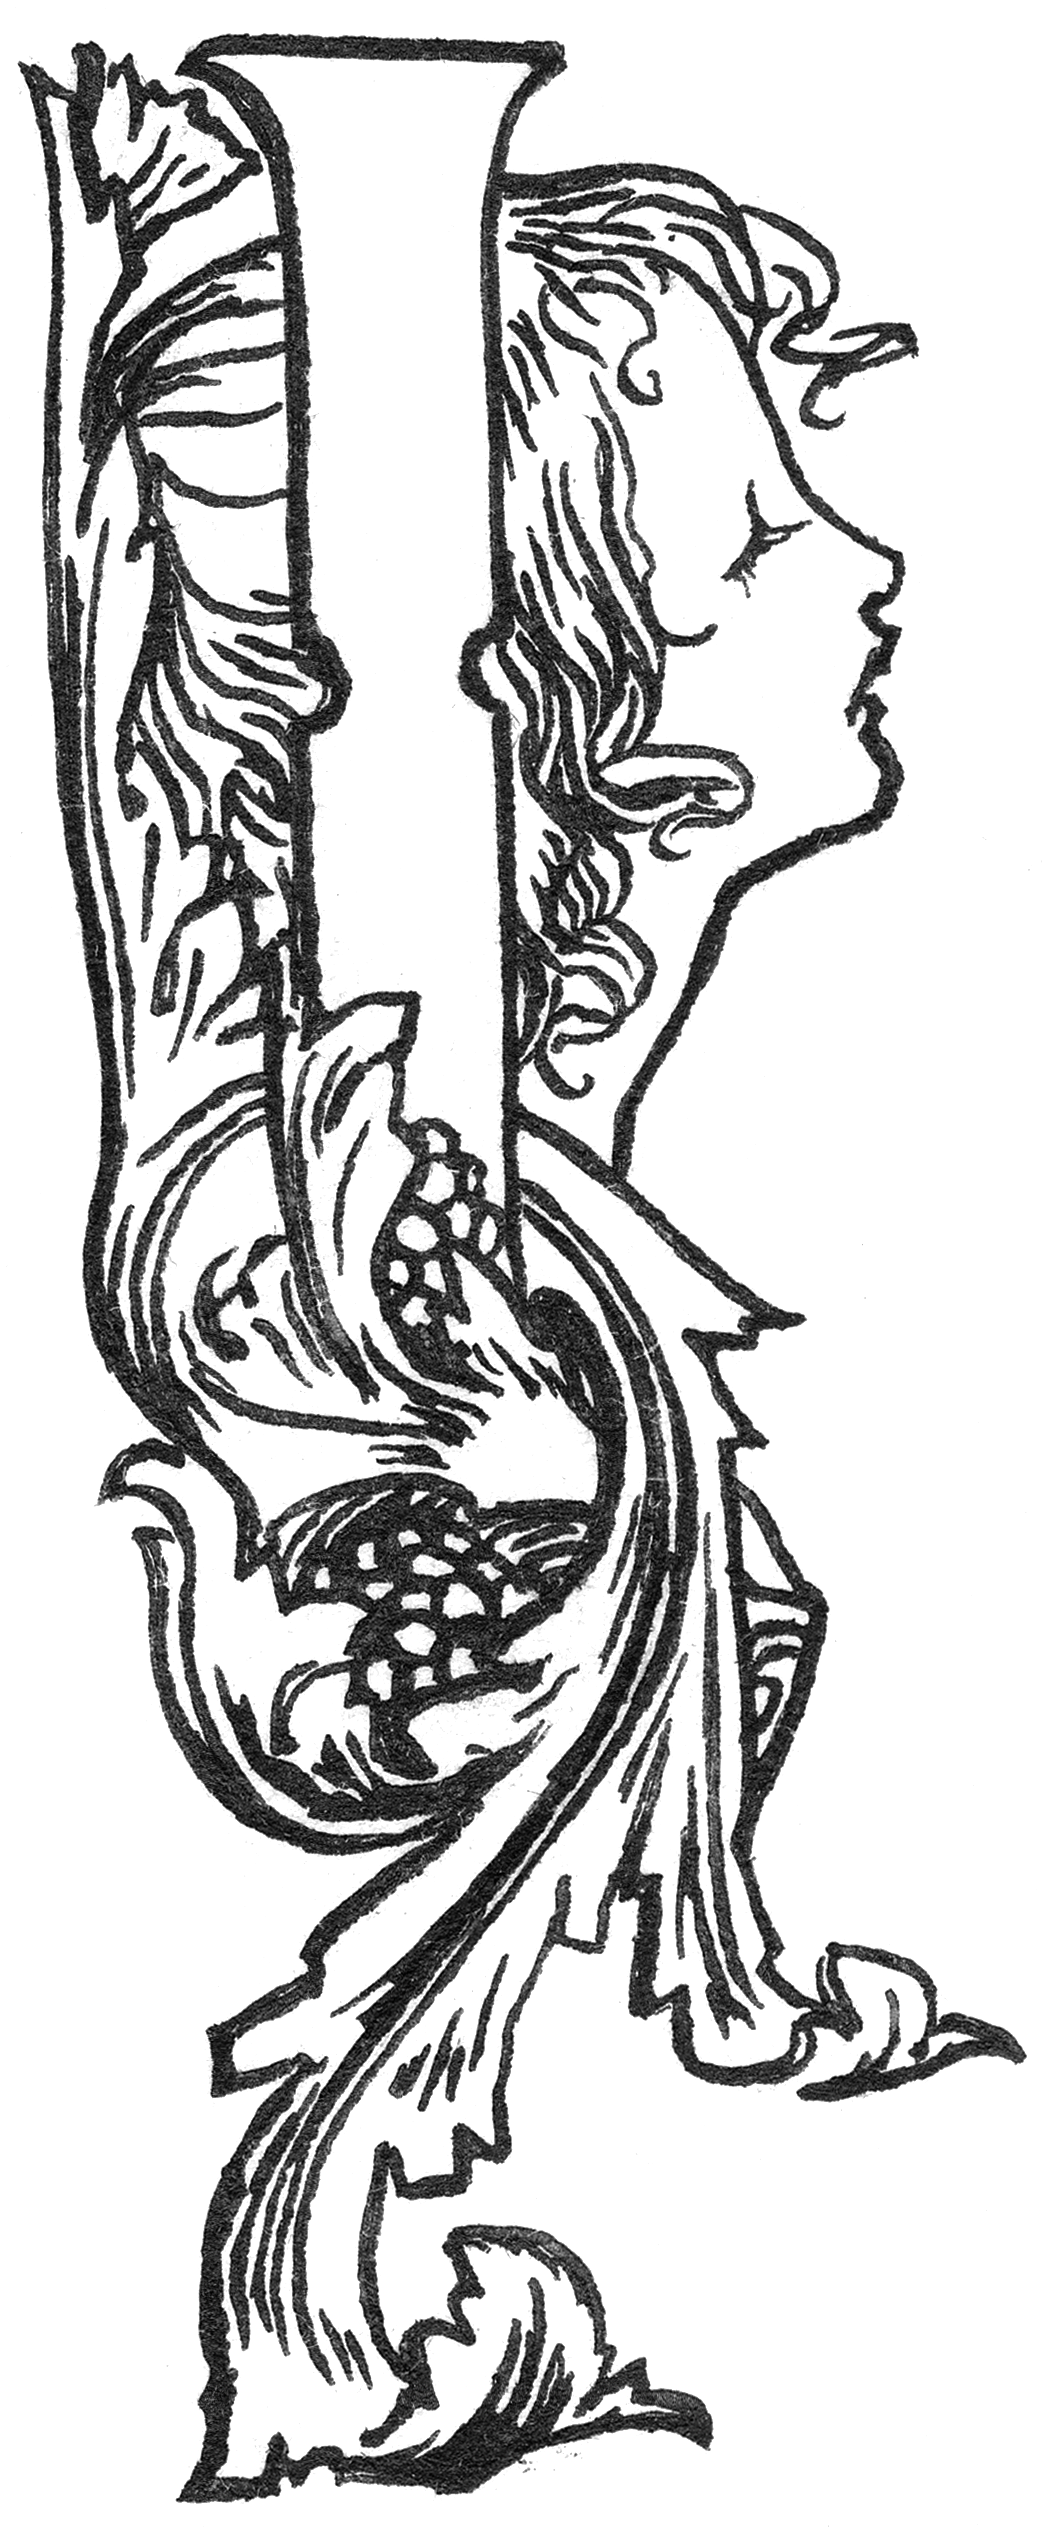
\includegraphics[width=0.125\linewidth]{4idropcapI}};
	\end{tikzpicture}
\end{a4}

\begin{verse_speech}[Prospero] 
\hspace{2em} f I have too austerely punish'd you,\\
\hspace{2.5em} Your compensation makes amends, for I\\
\hspace{2.5em} Have given you here a third of mine own life,\\
\hspace{2.5em} Or that for which I live; who once again\\
\hspace{2.5em} I tender to thy hand: all thy vexations\\
Were but my trials of thy love and thou\\
Hast strangely stood the test here, afore Heaven,\\
I ratify this my rich gift. O Ferdinand,\\
Do not smile at me that I boast her off,\\
For thou shalt find she will outstrip all praise\\
And make it halt behind her.
\end{verse_speech}

\begin{verse_speech}[Ferdinand] 
\hspace{\widthof{And make it halt behind her.}}I do believe it\\
Against an oracle.
\end{verse_speech}

\begin{verse_speech}[Prospero] 
Then, as my gift and thine own acquisition\\
Worthily purchased take my daughter: but\\
If thou dost break her virgin-knot before\\
All sanctimonious ceremonies may\\
With full and holy rite be minister'd,\\
No sweet aspersion shall the heavens let fall\\
To make this contract grow: but barren hate,\\
Sour-eyed disdain and discord shall bestrew\\
The union of your bed with weeds so loathly\\
That you shall hate it both: therefore take heed,\\
As Hymen's lamps shall light you.
\end{verse_speech}

\begin{verse_speech}[Ferdinand] 
\hspace{\widthof{As Hymen's lamps shall light you.}}As I hope\\
For quiet days, fair issue and long life,\\
With such love as 'tis now, the murkiest den,\\
The most opportune place, the strong'st suggestion.\\
Our worser genius can, shall never melt\\
Mine honour into lust, to take away\\
The edge of that day's celebration\\
When I shall think: or Phoebus' steeds are founder'd,\\
Or Night kept chain'd below.
\end{verse_speech}

\begin{verse_speech}[Prospero] 
\hspace{\widthof{Or Night kept chain'd below.}}Fairly spoke.\\
Sit then and talk with her; she is thine own.\\
What, Ariel! my industrious servant, Ariel!
\end{verse_speech}

\enter{\textsc{Ariel}}

\verseline[Ariel]{What would my potent master? here I am.}

\begin{verse_speech}[Prospero] 
Thou and thy meaner fellows your last service\\
Did worthily perform; and I must use you\\
In such another trick. Go bring the rabble,\\
O'er whom I give thee power, here to this place:\\
Incite them to quick motion; for I must\\
Bestow upon the eyes of this young couple\\
Some vanity of mine art: it is my promise,\\
And they expect it from me.
\end{verse_speech}

\verseline[Ariel]{\hspace{\widthof{And they expect it from me.}}Presently?}

\verseline[Prospero]{Ay, with a twink.}

\begin{verse_speech}[Ariel] 
	\begin{song}
\songline{Before you can say <come> and <go,>}
\songline{And breathe twice and cry <so, so,>}
\songline{Each one, tripping on his toe,}
\songline{Will be here with mop and mow.}
\songline{Do you love me, master? no?}
\end{song}
\end{verse_speech}

% \begin{figure}[tb]
% \centering
% 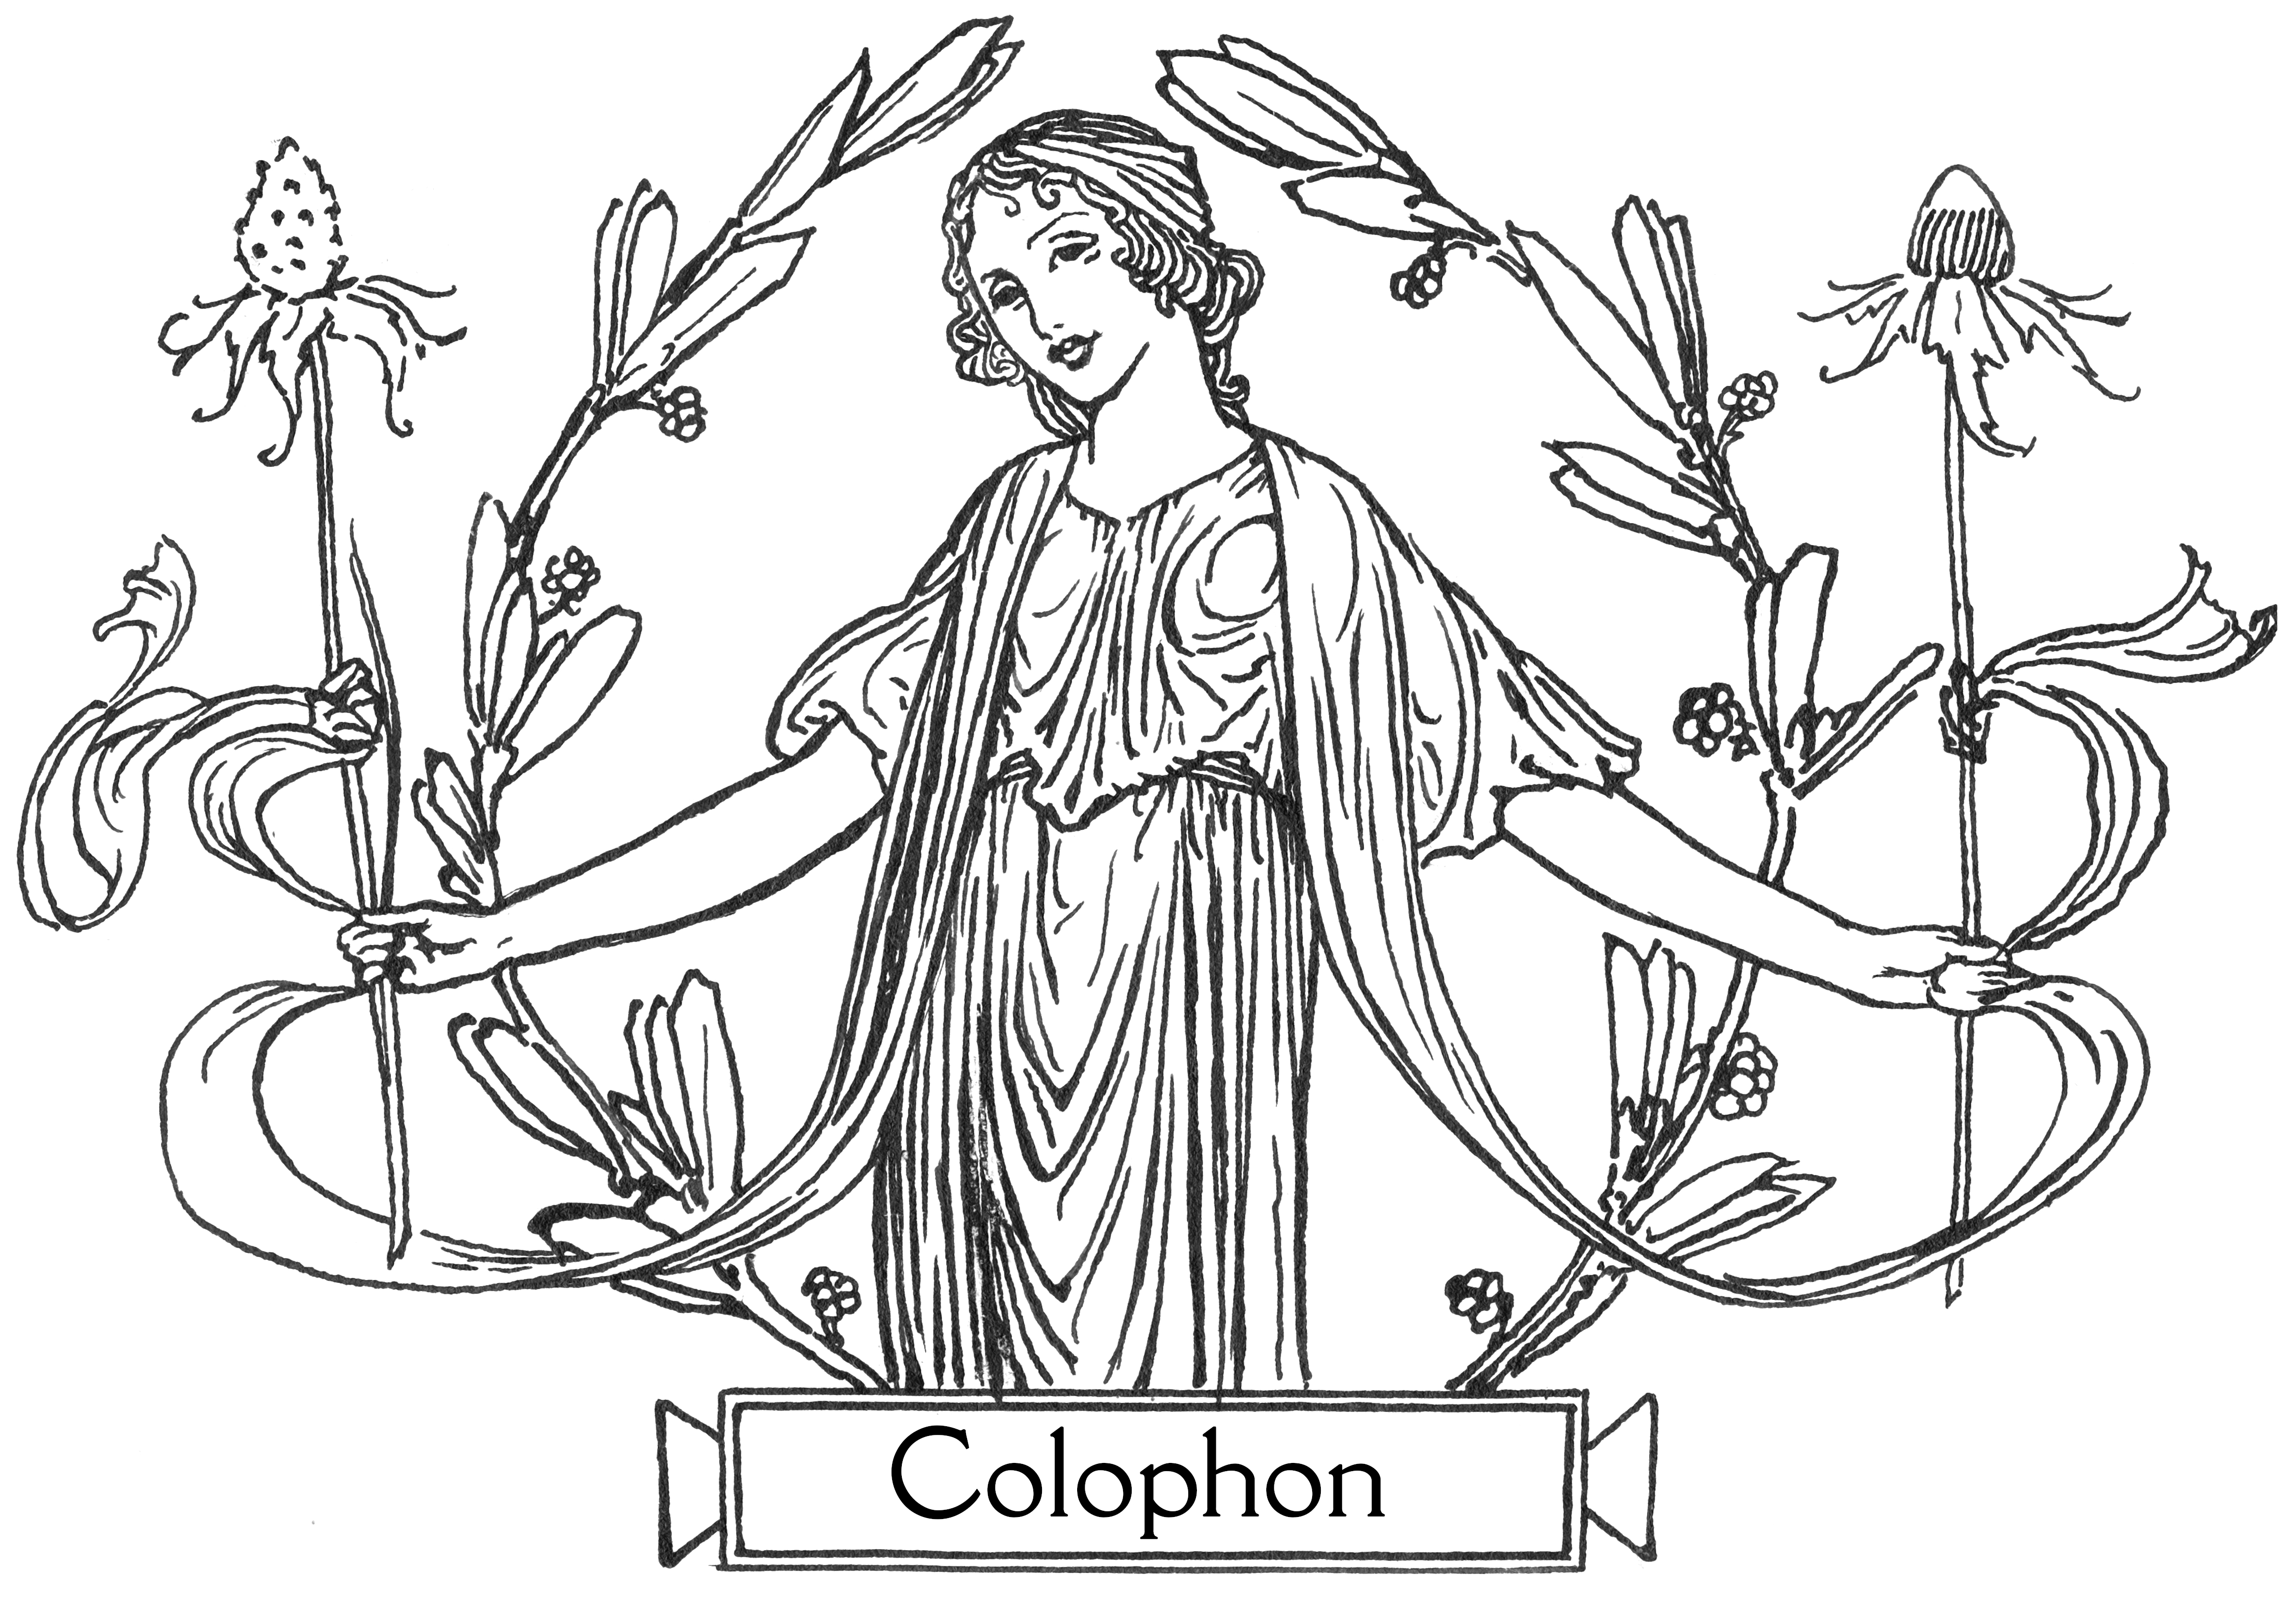
\includegraphics[width=.8\textwidth]{4iflowerlady}
% \end{figure}

\begin{verse_speech}[Prospero] 
Dearly my delicate Ariel. Do not approach\\
Till thou dost hear me call.
\end{verse_speech}

\verseline[Ariel]{\hspace{\widthof{Till thou dost hear me call.}}Well, I conceive.}

\stage{He exits.}

\begin{verse_speech}[Prospero] 
Look thou be true; do not give dalliance\\
Too much the rein: the strongest oaths are straw\\
To the fire i' the blood: be more abstemious,\\
Or else, good night your vow!
\end{verse_speech}

\begin{verse_speech}[Ferdinand] 
\hspace{\widthof{Or else, good night your vow!}}I warrant you, sir;\\
The white cold virgin snow upon my heart\\
Abates the ardour of my liver.
\end{verse_speech}

\begin{verse_speech}[Prospero] 
\hspace{\widthof{Abates the ardour of my liver.}}Well.\\
Now come, my Ariel! bring a corollary,\\
Rather than want a spirit: appear and pertly!\\
No tongue! all eyes! be silent.
\end{verse_speech}

	\begin{bwbigpic}
		[\picwidth]
		{4imasqueleft}
		{}
	\end{bwbigpic}

\stage{Soft music. Enter \textsc{Iris}.}

\begin{verse_speech}[Iris] 
Ceres, most bounteous lady, thy rich leas\\
Of wheat, rye, barley, vetches, oats and pease;\\
Thy turfy mountains, where live nibbling sheep,\\
And flat meads thatch'd with stover, them to keep;\\
Thy banks with pioned and twilled brims,\\
Which spongy April at thy hest betrims,\\
To make cold nymphs chaste crowns; and thy broom-groves,\\
Whose shadow the dismissed bachelor loves,\\
Being lass-lorn: thy pole-clipt vineyard;\\
And thy sea-marge, sterile and rocky-hard,\\
Where thou thyself dost air;—the queen o' the sky,\\
Whose watery arch and messenger am I,\\
Bids thee leave these, and with her sovereign grace,\\
Here on this grass-plot, in this very place,\\
To come and sport: her peacocks fly amain:\\
Approach, rich Ceres, her to entertain.
\end{verse_speech}

\enter{\textsc{Ceres}}

\begin{verse_speech}[Ceres] 
Hail, many-colour'd messenger, that ne'er\\
Dost disobey the wife of Jupiter;\\
Who with thy saffron wings upon my flowers\\
Diffusest honey-drops, refreshing showers,\\
And with each end of thy blue bow dost crown\\
My bosky acres and my unshrubb'd down,\\
Rich scarf to my proud earth; why hath thy queen\\
Summon'd me hither, to this short-grass'd green?
\end{verse_speech}


	\begin{bwbigpic}
		[\picwidth]
		{4imasqueright}
		{}
	\end{bwbigpic}



\begin{verse_speech}[Iris] 
A contract of true love to celebrate;\\
And some donation freely to estate\\
On the blest lovers.
\end{verse_speech}

\begin{verse_speech}[Ceres] 
\hspace{\widthof{On the blest lovers.}}Tell me, heavenly bow,\\
If Venus or her son, as thou dost know,\\
Do now attend the queen? Since they did plot\\
The means that dusky Dis my daughter got,\\
Her and her blind boy's scandal'd company\\
I have forsworn.
\end{verse_speech}


\begin{verse_speech}[Iris] 
\hspace{\widthof{I have forsworn.}}Of her society\\
Be not afraid: I met her deity\\
Cutting the clouds towards Paphos and her son\\
Dove-drawn with her. Here thought they to have done\\
Some wanton charm upon this man and maid,\\
Whose vows are, that no bed-right shall be paid\\
Till Hymen's torch be lighted: but vain;\\
Mars's hot minion is returned again;\\
Her waspish-headed son has broke his arrows,\\
Swears he will shoot no more but play with sparrows\\
And be a boy right out.
\end{verse_speech}


\begin{verse_speech}[Ceres] 
\hspace{\widthof{And be a boy right out.}}High'st queen of state,\\
Great Juno, comes; I know her by her gait.
\end{verse_speech}

\enter{\textsc{Juno}}

\begin{verse_speech}[Juno] 
How does my bounteous sister? Go with me\\
To bless this twain, that they may prosperous be\\
And honour'd in their issue.
\end{verse_speech}

\stage{They sing:}

\begin{verse_speech}[Juno]
	\begin{song}
\songline{Honour, riches, marriage-blessing,}
\songline{Long continuance, and increasing,}
\songline{Hourly joys be still upon you!}
\songline{Juno sings her blessings upon you.}
\end{song}
\end{verse_speech}

\begin{verse_speech}[Ceres] 
	\begin{song}
\songline{Earth's increase, foison plenty,}
\songline{Barns and garners never empty,}
\songline{Vines and clustering bunches growing,}
\songline{Plants with goodly burthen bowing;}
\songline{Spring come to you at the farthest}
\songline{In the very end of harvest!}
\songline{Scarcity and want shall shun you;}
\songline{Ceres' blessing so is on you.}
\end{song}
\end{verse_speech}


\begin{verse_speech}[Ferdinand] 
This is a most majestic vision, and\\
Harmoniously charmingly. May I be bold\\
To think these spirits?
\end{verse_speech}


\begin{verse_speech}[Prospero] 
\hspace{\widthof{To think these spirits?}}Spirits, which by mine art\\
I have from their confines call'd to enact\\
My present fancies.
\end{verse_speech}

\begin{verse_speech}[Ferdinand] 
\hspace{\widthof{My present fancies.}}Let me live here ever;\\
So rare a wonder'd father and a wife\\
Makes this place Paradise.
\end{verse_speech}

\stage{\textsc{Juno} and \textsc{Ceres} whisper, and send \textsc{Iris} on employment.}

\begin{verse_speech}[Prospero] 
\hspace{\widthof{Makes this place Paradise.}}Sweet, now, silence!\\
Juno and Ceres whisper seriously;\\
There's something else to do: hush, and be mute,\\
Or else our spell is marr'd.
\end{verse_speech}

\begin{verse_speech}[Iris] 
You nymphs, call'd Naiads, of the windring brooks,\\
With your sedged crowns and ever-harmless looks,\\
Leave your crisp channels and on this green land\\
Answer your summons; Juno does command:\\
Come, temperate nymphs, and help to celebrate\\
A contract of true love; be not too late.\\
\enter{certain Nymphs}
You sunburnt sicklemen, of August weary,\\
Come hither from the furrow and be merry:\\
Make holiday; your rye-straw hats put on\\
And these fresh nymphs encounter every one\\
In country footing.
\end{verse_speech}

\enter{certain Reapers, properly habited: they join with the Nymphs in a graceful dance; towards the end whereof \textsc{Prospero} starts suddenly, and speaks; after which, to a strange, hollow, and confused noise, they heavily vanish}

\begin{verse_speech}[Prospero] 
	\aside{I had forgot that foul conspiracy\\
Of the beast Caliban and his confederates\\
Against my life: the minute of their plot\\
Is almost come.}
\stage{To the Spirits}
Well done! avoid; no more!
\end{verse_speech}

\begin{verse_speech}[Ferdinand] 
This is strange: your father's in some passion\\
That works him strongly.
\end{verse_speech}

\begin{verse_speech}[Miranda] 
\hspace{\widthof{That works him strongly.}}Never till this day\\
Saw I him touch'd with anger so distemper'd.
\end{verse_speech}

\begin{verse_speech}[Prospero] 
You do look, my son, in a moved sort,\\
As if you were dismay'd: be cheerful, sir.\\
Our revels now are ended. These our actors,\\
As I foretold you, were all spirits and\\
Are melted into air, into thin air:\\
And, like the baseless fabric of this vision,\\
The cloud-capp'd towers, the gorgeous palaces,\\
The solemn temples, the great globe itself,\\
Ye all which it inherit, shall dissolve\\
And, like this insubstantial pageant faded,\\
Leave not a rack behind. We are such stuff\\
As dreams are made on, and our little life\\
Is rounded with a sleep. Sir, I am vex'd;\\
Bear with my weakness; my, brain is troubled:\\
Be not disturb'd with my infirmity:\\
If you be pleased, retire into my cell\\
And there repose: a turn or two I'll walk,\\
To still my beating mind.
\end{verse_speech}

\verseline[Ferdinand]{\textit{[With Miranda]}\hspace{\widthof{To still my beating mind.}-\widthof{[With Miranda]}} We wish your peace.}

\exeunt{}

\verseline[Prospero]{Come with a thought I thank thee, Ariel: come.}
\enter{\textsc{Ariel}}

\verseline[Ariel]{Thy thoughts I cleave to. What's thy pleasure?}


\begin{verse_speech}[Prospero] 
\hspace{\widthof{Thy thoughts I cleave to. What's thy pleasure?}}Spirit,\\
We must prepare to meet with Caliban.
\end{verse_speech}

\begin{verse_speech}[Ariel] 
Ay, my commander: when I presented Ceres,\\
I thought to have told thee of it, but I fear'd\\
Lest I might anger thee.
\end{verse_speech}

\verseline[Prospero]{Say again, where didst thou leave these varlets?}

\begin{verse_speech}[Ariel] 
I told you, sir, they were red-hot with drinking;\\
So fun of valour that they smote the air\\
For breathing in their faces; beat the ground\\
For kissing of their feet; yet always bending\\
Towards their project. Then I beat my tabour;\\
At which, like unback'd colts, they prick'd their ears,\\
Advanced their eyelids, lifted up their noses\\
As they smelt music: so I charm'd their ears\\
That calf-like they my lowing follow'd through\\
Tooth'd briers, sharp furzes, pricking goss and thorns,\\
Which entered their frail shins: at last I left them\\
I' the filthy-mantled pool beyond your cell,\\
There dancing up to the chins, that the foul lake\\
O'erstunk their feet.
\end{verse_speech}

\begin{verse_speech}[Prospero] 
\hspace{\widthof{O'erstunk their feet.}}This was well done, my bird.\\
Thy shape invisible retain thou still:\\
The trumpery in my house, go bring it hither,\\
For stale to catch these thieves.
\end{verse_speech}

\verseline[Ariel]{\hspace{\widthof{For stale to catch these thieves.}}I go, I go.}

\exit{}

\begin{verse_speech}[Prospero] 
A devil, a born devil, on whose nature\\
Nurture can never stick; on whom my pains,\\
Humanely taken, all, all lost, quite lost;\\
And as with age his body uglier grows,\\
So his mind cankers. I will plague them all,\\
Even to roaring.

\stage{Re-enter \textsc{Ariel}, loaden with glistering apparel, \&c}

Come, hang them on this line.

\end{verse_speech}

	\begin{bwbigpic}
		[\picwidth]
		{4iwashing}
		{}
	\end{bwbigpic}

\stage{\textsc{Prospero} and \textsc{Ariel} remain invisible. Enter \textsc{Caliban}, \textsc{Stephano}, and \textsc{Trinculo}, all wet}

\begin{verse_speech}[Caliban] 
Pray you, tread softly, that the blind mole may not\\
Hear a foot fall: we now are near his cell.
\end{verse_speech}

\verseline[Stephano]{Monster, your fairy, which you say is a harmless fairy, has done little better than played the Jack with us.}

\verseline[Trinculo]{Monster, I do smell all horse-piss; at which my nose is in great indignation.}

\verseline[Stephano]{So is mine. Do you hear, monster? If I should take a displeasure against you, look you,—}

\verseline[Trinculo]{Thou wert but a lost monster.}

\begin{verse_speech}[Caliban] 
Good my lord, give me thy favour still.\\
Be patient, for the prize I'll bring thee to\\
Shall hoodwink this mischance: therefore speak softly.\\
All's hush'd as midnight yet.
\end{verse_speech}

\verseline[Trinculo]{Ay, but to lose our bottles in the pool,—}

\verseline[Stephano]{There is not only disgrace and dishonour in that, monster, but an infinite loss.}

\verseline[Trinculo]{That's more to me than my wetting: yet this is your harmless fairy, monster.}

\verseline[Stephano]{I will fetch off my bottle, though I be o'er ears for my labour.}

\begin{verse_speech}[Caliban] 
Prithee, my king, be quiet. Seest thou here,\\
This is the mouth o' the cell: no noise, and enter.\\
Do that good mischief which may make this island\\
Thine own for ever, and I, thy Caliban,\\
For aye thy foot-licker.
\end{verse_speech}

\verseline[Stephano]{Give me thy hand. I do begin to have bloody thoughts.}

\verseline[Trinculo]{\textit{(Seeing the apparel)} O king Stephano! O peer! O worthy Stephano! look what a wardrobe here is for thee!}

\verseline[Caliban]{Let it alone, thou fool; it is but trash.}

\begin{prose_speech}[Trinculo]
O, ho, monster! we know what belongs to a frippery.
\stage{He puts on one of the gowns.}
O king Stephano!
\end{prose_speech}

\verseline[Stephano]{Put off that gown, Trinculo; by this hand, I'll have that gown.}

\verseline[Trinculo]{Thy grace shall have it.}

\begin{verse_speech}[Caliban] 
The dropsy drown this fool! What do you mean\\
To dote thus on such luggage? Let's alone\\
And do the murder first: if he awake,\\
From toe to crown he'll fill our skins with pinches,\\
Make us strange stuff.
\end{verse_speech}

\begin{prose_speech}[Stephano]
Be you quiet, monster. Mistress line, is not this my jerkin? 

\stage{He takes a jacket from the tree.}

Now is the jerkin under the line: now, jerkin, you are like to lose your hair and prove a bald jerkin.
\end{prose_speech}


\verseline[Trinculo]{Do, do: we steal by line and level, an't like your grace.}

\verseline[Stephano]{I thank thee for that jest; here's a garment for't: wit shall not go unrewarded while I am king of this country. <Steal by line and level> is an excellent pass of pate; there's another garment for't.}

\verseline[Trinculo]{Monster, come, put some lime upon your fingers, and away with the rest.}
	
\begin{verse_speech}[Caliban] 
I will have none on't: we shall lose our time,\\
And all be turn'd to barnacles, or to apes\\
With foreheads villanous low.
\end{verse_speech}

\verseline[Stephano]{Monster, lay-to your fingers: help to bear this away where my hogshead of wine is, or I'll turn you out of my kingdom: go to, carry this.}

\verseline[Trinculo]{And this.}

\verseline[Stephano]{Ay, and this.}

\stage{A noise of hunters heard. Enter divers Spirits, in shape of dogs and hounds, and hunt them about, \textsc{Prospero} and \textsc{Ariel} setting them on.}

\verseline[Prospero]{Hey, Mountain, hey!}

\verseline[Ariel]{Silver I there it goes, Silver!}

\begin{verse_speech}[Prospero] 
Fury, Fury! there, Tyrant, there! hark! hark!
	
\stage{\textsc{Caliban}, \textsc{Stephano}, and \textsc{Trinculo} are driven off}

Go charge my goblins that they grind their joints\\
With dry convulsions, shorten up their sinews\\
With agèd cramps, and more pinch-spotted make them\\
Than pard or cat o' mountain.
\end{verse_speech}

\verseline[Ariel]{\hspace{\widthof{Than pard or cat o' mountain.}}Hark, they roar!}

\begin{verse_speech}[Prospero] 
Let them be hunted soundly. At this hour\\
Lie at my mercy all mine enemies:\\
Shortly shall all my labours end, and thou\\
Shalt have the air at freedom: for a little\\
Follow, and do me service.
\end{verse_speech}

\exeunt{}

\vfill

\begin{center}
	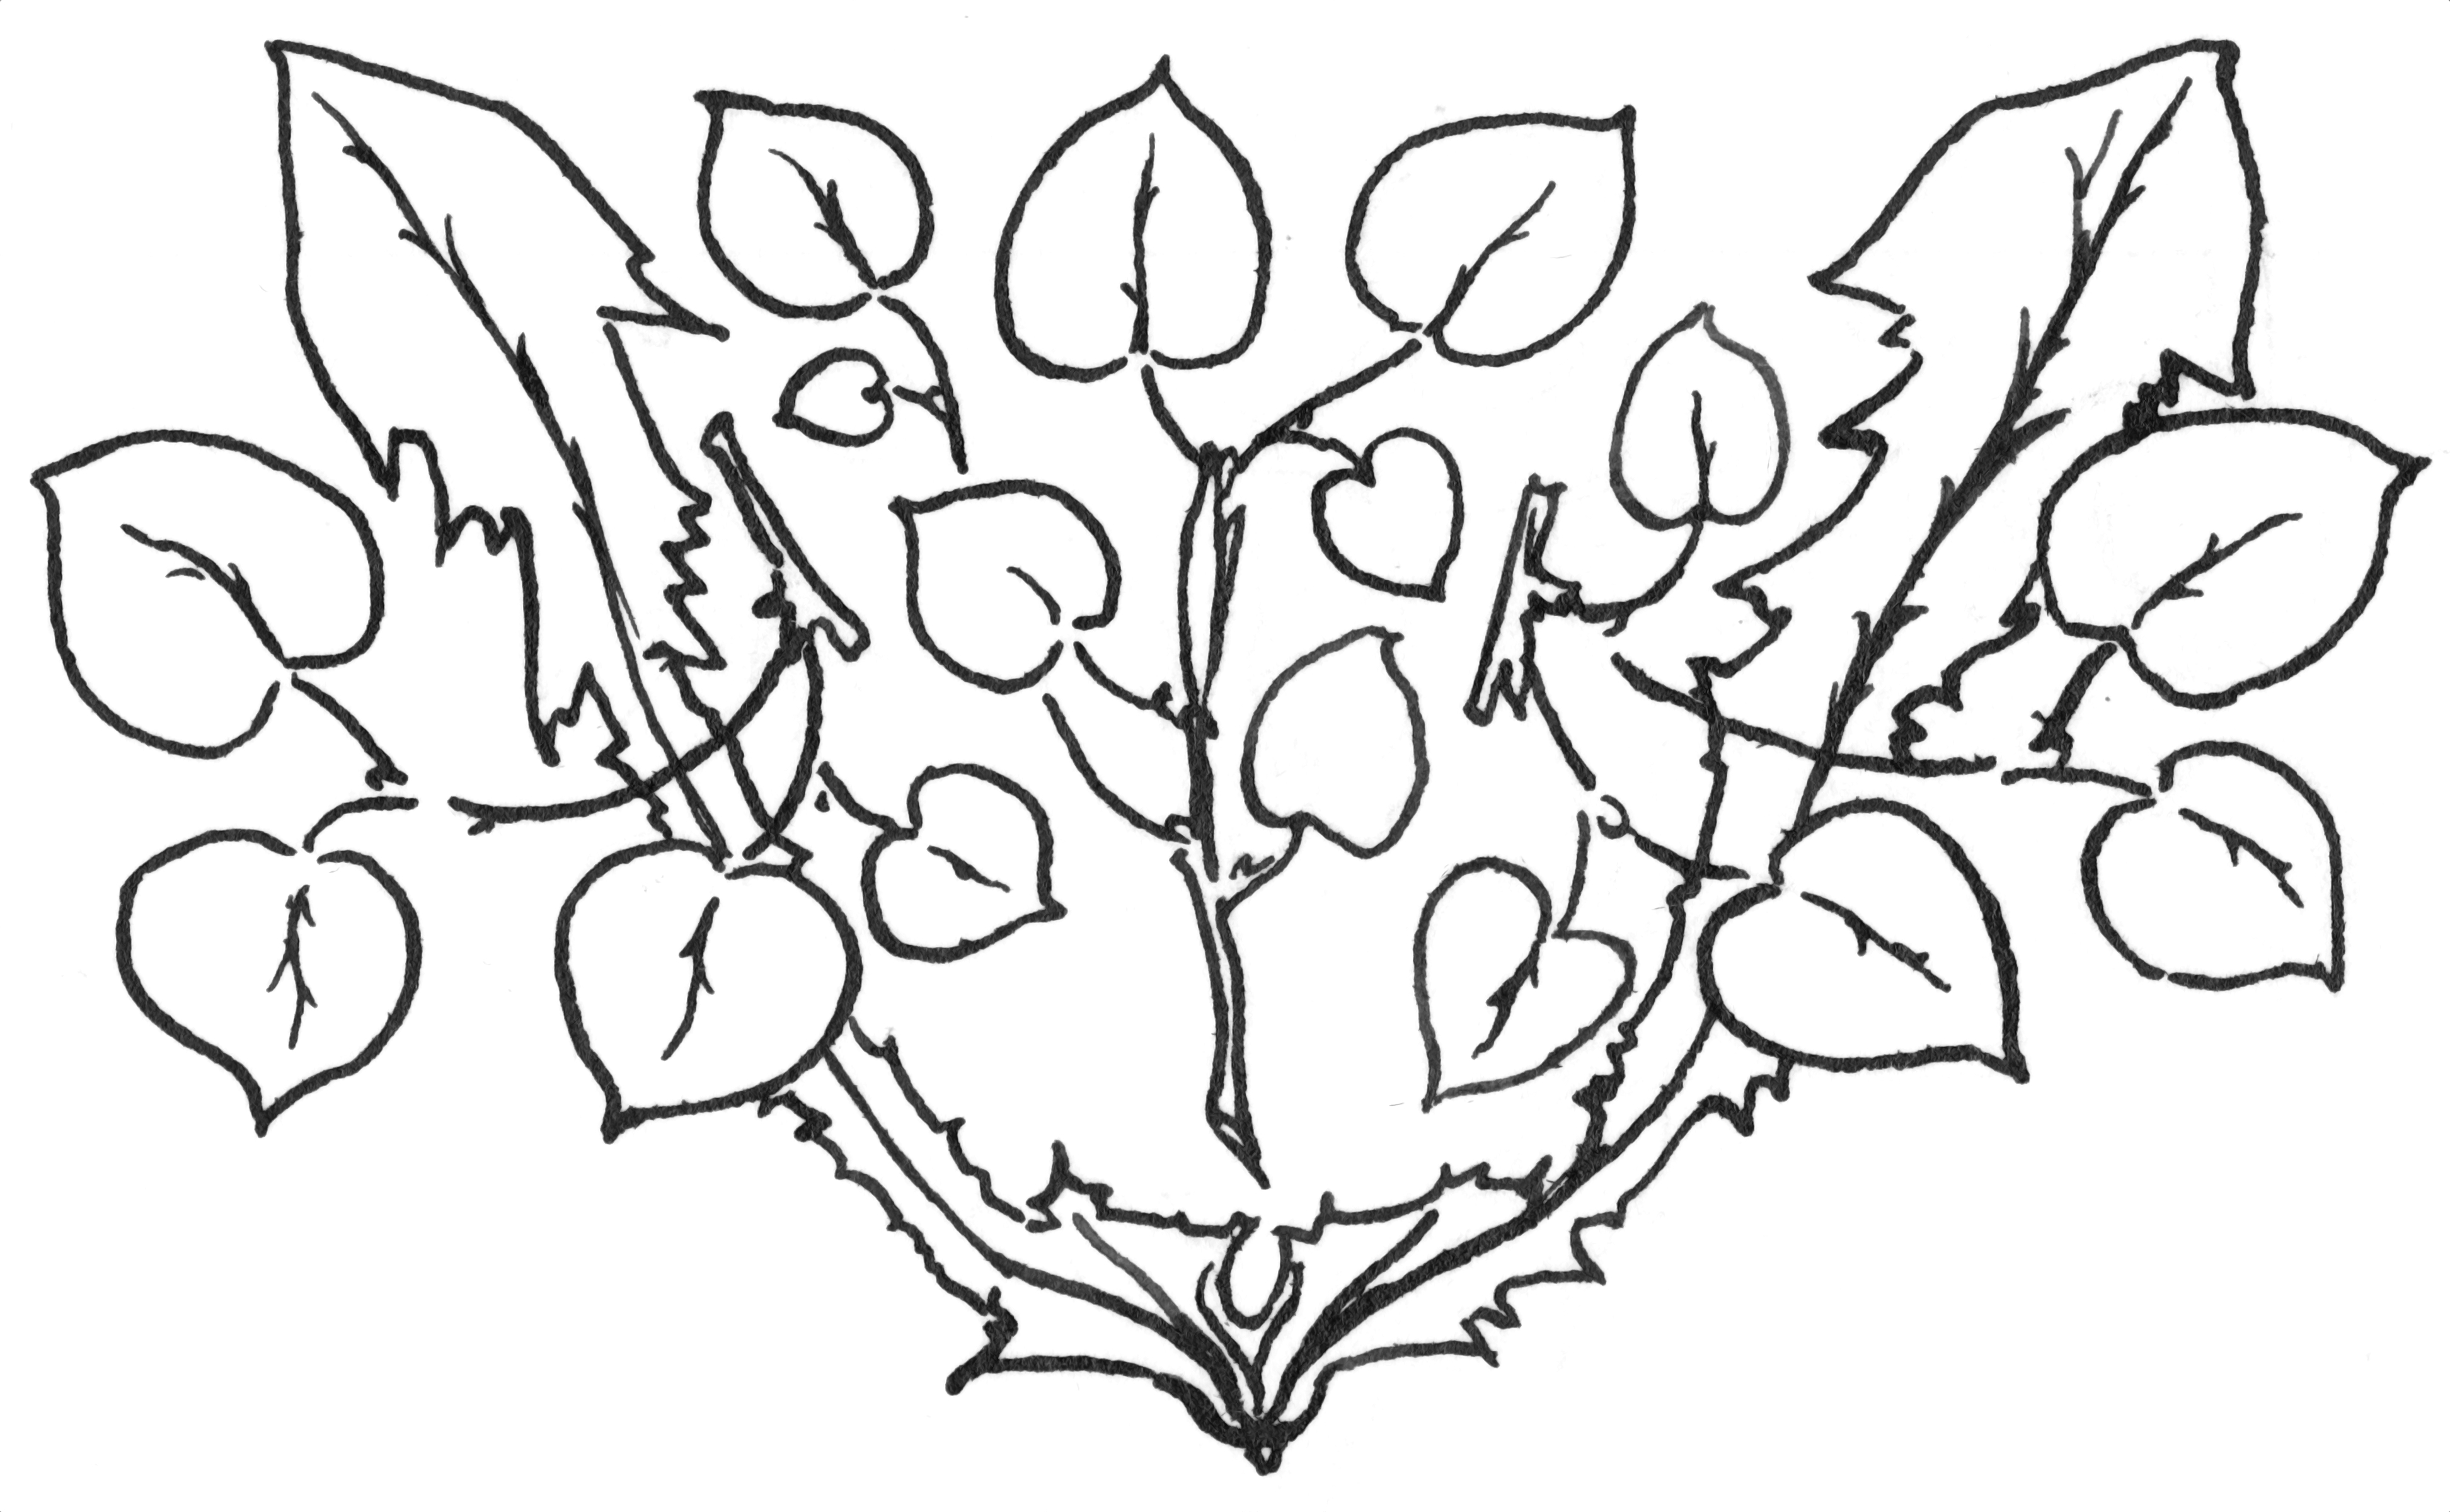
\includegraphics[width=.4\textwidth]{3iitailpiece}

\end{center}